\begin{table}[ht]
	\begin{Dtabular}[1.1]{|c|c|c|c|}
		\hline
		CSV File&Parameter $m$&Parameter $b$&$d_s$\\
		\hline
		\verb|lockin_2|&$0.01090\pm0.00011$&$-8.16\pm0.08$&$748\pm11 $\\
		\hline
		\verb|lockin_3|&$0.01091\pm0.00011$&$-3.74\pm0.04$&$1022\pm22$ \\
		\hline
		\verb|lockin_4|&$0.01093\pm0.00016$&$-11.16\pm0.16$&$518\pm8$\\
		\hline
		\verb|lockin_5|&$0.01090\pm0.00010$&$-5.65\pm0.06$&$945\pm17$\\
		\hline
		\verb|lockin_6|&$0.01092\pm0.00013$&$-10.32\pm0.12$&$375\pm6$\\
		\hline
		\verb|lockin_7|&$0.01094\pm0.00011$&$-4.10\pm0.04$&$472\pm7$\\
		\hline
		\verb|lockin_8|&$0.01090\pm0.00010$&$-5.14\pm0.05$&$355\pm5$\\
		\hline
		\verb|lockin_8|&$0.01091\pm0.00011$&$-3.87\pm0.04$&$355\pm5$\\
		\hline
	\end{Dtabular}
	\centering
	\caption[Parameter of Sawtooth]{Parameters and position of the 'Nulldurchgang' of the sawtooth fit. Here $m$ is the slope, $b$ the crossing of the y-axis and $d_s$ the 'Nulldurchgang'.}
	\label{SägezahnParameter}
	\end{table}
	\begin{figure}[ht]
		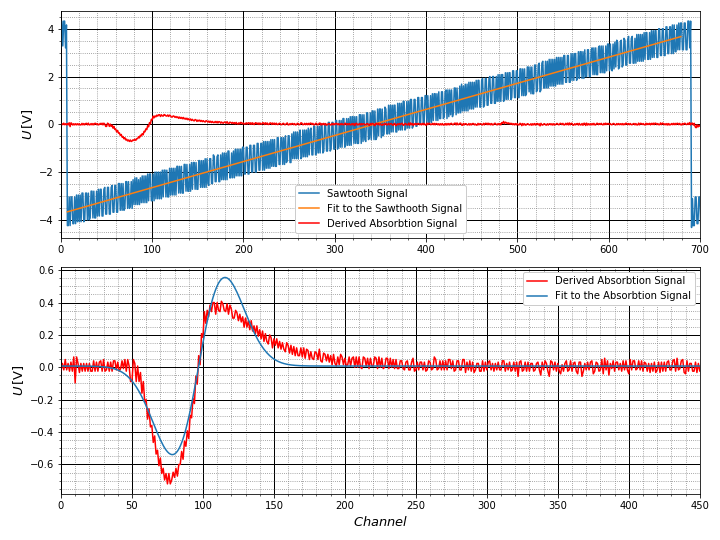
\includegraphics[scale=0.5]{Bild/LockIn2.png}
		\centering
		\caption[Plots and Fits of Lock-In Method 2]{\small The upper figure shows the data of the sawtooth in blue with the corresponding fit in orange. The absorption signal is in red. The lower one shows the part of the absorption signal which is of interest with the fit in blue. This figure is of the CSV file lockin 2.}
		\label{Lock2}
	\end{figure}
	\begin{figure}[ht]
		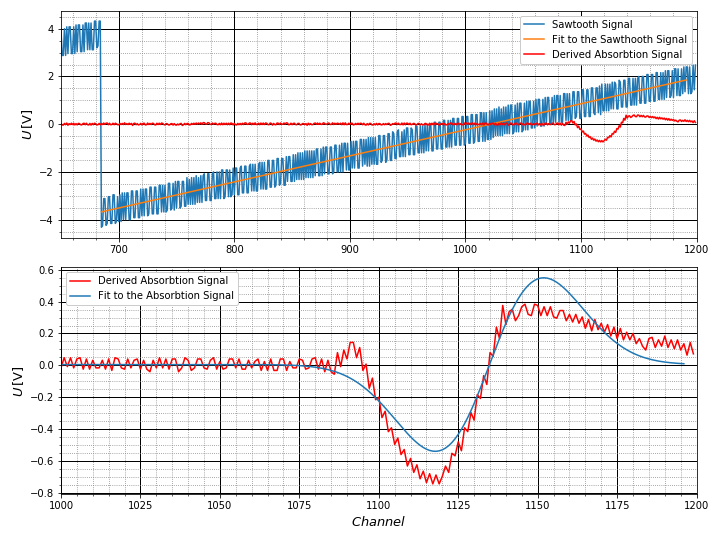
\includegraphics[scale=0.5]{Bild/LockIn3.png}
		\centering
		\caption[Plots and Fits of Lock-In Method 3]{\small The upper figure shows the data of the sawtooth in blue with the corresponding fit in orange. The absorption signal is in red. The lower one shows the part of the absorption signal which is of interest with the fit in blue. This figure is of the CSV file lockin 3.}
		\label{Lock3}
	\end{figure}
	\begin{figure}[ht]
		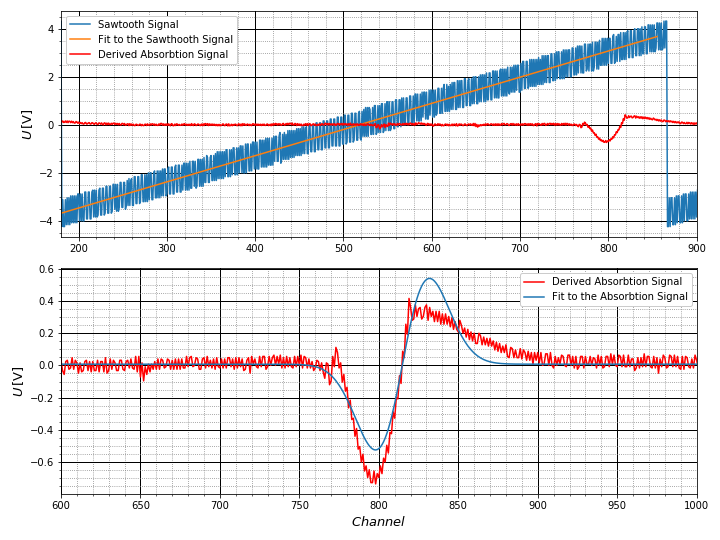
\includegraphics[scale=0.5]{Bild/LockIn4.png}
		\centering
		\caption[Plots and Fits of Lock-In Method 4]{\small The upper figure shows the data of the sawtooth in blue with the corresponding fit in orange. The absorption signal is in red. The lower one shows the part of the absorption signal which is of interest with the fit in blue. This figure is of the CSV file lockin 4.}
		\label{Lock4}
	\end{figure}
	\begin{figure}[ht]
		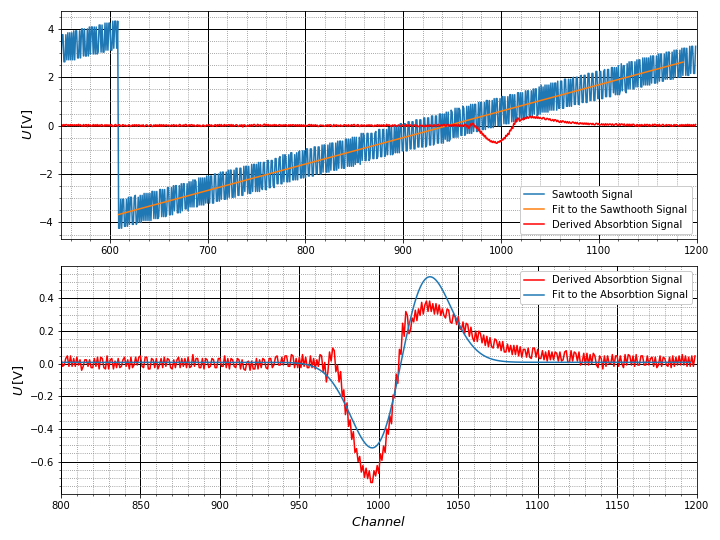
\includegraphics[scale=0.5]{Bild/LockIn5.png}
		\centering
		\caption[Plots and Fits of Lock-In Method 5]{\small The upper figure shows the data of the sawtooth in blue with the corresponding fit in orange. The absorption signal is in red. The lower one shows the part of the absorption signal which is of interest with the fit in blue. This figure is of the CSV file lockin 5.}
		\label{Lock5}
	\end{figure}
	\begin{figure}[ht]
		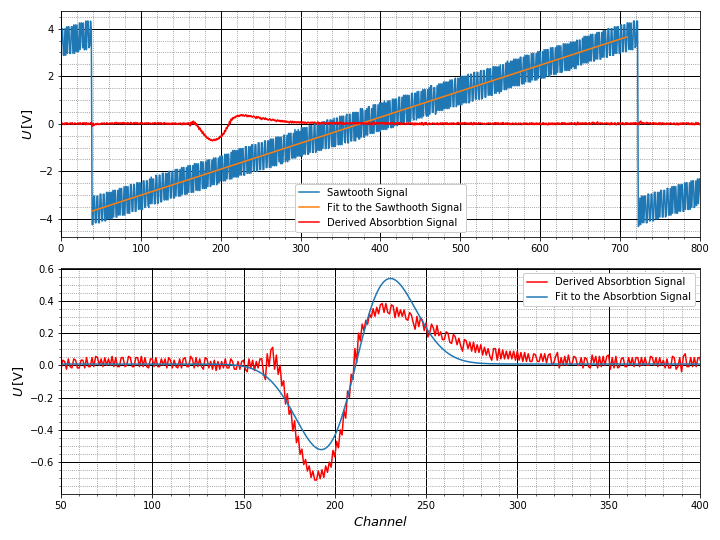
\includegraphics[scale=0.5]{Bild/LockIn6.png}
		\centering
		\caption[Plots and Fits of Lock-In Method 6]{\small The upper figure shows the data of the sawtooth in blue with the corresponding fit in orange. The absorption signal is in red. The lower one shows the part of the absorption signal which is of interest with the fit in blue. This figure is of the CSV file lockin 6.}
		\label{Lock6}
	\end{figure}
	\begin{figure}[ht]
		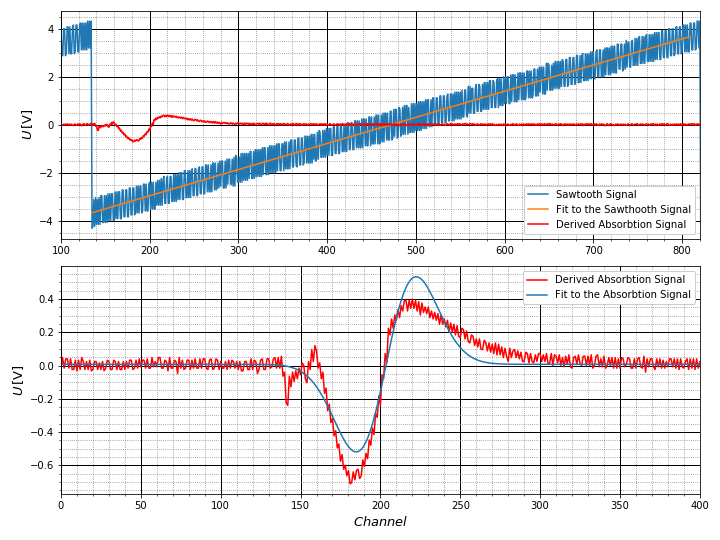
\includegraphics[scale=0.5]{Bild/LockIn7.png}
		\centering
		\caption[Plots and Fits of Lock-In Method 7]{\small The upper figure shows the data of the sawtooth in blue with the corresponding fit in orange. The absorption signal is in red. The lower one shows the part of the absorption signal which is of interest with the fit in blue. This figure is of the CSV file lockin 7.}
		\label{Lock7}
	\end{figure}
